\begin{center}
    \(
    \begin{tikzcd}
    
\begin{tikzpicture}[x=2em, y=2em, baseline=0.7em]
        \draw[very thick, black!50] (0,0)--(1,0)--(1,1)--(0,1)--(0,0);
        \filldraw (0,0) circle (2pt);
    \end{tikzpicture}
    \ar[r, hook]\ar[d]
    & 
    
\begin{tikzpicture}[x=2em, y=2em, baseline=0.7em]
        \draw[very thick] (0,0)--(1,0)--(1,1)--(0,1)--(0,0);
    \end{tikzpicture} 
    \ar[r, hook]\ar[d]
    &
    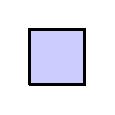
\begin{tikzpicture}[x=2em, y=2em, baseline=0.7em]
        \filldraw[very thick, fill=blue!20] (0,0)--(1,0)--(1,1)--(0,1)--(0,0);
    \end{tikzpicture}
    \ar[d]\\
    p(x)\ar[r, hook]&Y\ar[r, hook]&B
    \end{tikzcd}
    \)
\end{center}